%
% This is the LaTeX template file for lecture notes for EE 382C/EE 361C.
%
% To familiarize yourself with this template, the body contains
% some examples of its use.  Look them over.  Then you can
% run LaTeX on this file.  After you have LaTeXed this file then
% you can look over the result either by printing it out with
% dvips or using xdvi.
%
% This template is based on the template for Prof. Sinclair's CS 270.

\documentclass[twoside]{article}
\usepackage{graphics}
\usepackage{amsmath}
\usepackage{algorithm}
\usepackage[noend]{algpseudocode}
\usepackage{listings}
\usepackage{tabu}
\usepackage{graphicx}
\setlength{\oddsidemargin}{0.25 in}
\setlength{\evensidemargin}{-0.25 in}
\setlength{\topmargin}{-0.6 in}
\setlength{\textwidth}{6.5 in}
\setlength{\textheight}{8.5 in}
\setlength{\headsep}{0.75 in}
\setlength{\parindent}{0 in}
\setlength{\parskip}{0.1 in}

%
% The following commands set up the lecnum (lecture number)
% counter and make various numbering schemes work relative
% to the lecture number.
%
\newcounter{lecnum}
\renewcommand{\thepage}{\thelecnum-\arabic{page}}
\renewcommand{\thesection}{\thelecnum.\arabic{section}}
\renewcommand{\theequation}{\thelecnum.\arabic{equation}}
\renewcommand{\thefigure}{\thelecnum.\arabic{figure}}
\renewcommand{\thetable}{\thelecnum.\arabic{table}}

%
% The following macro is used to generate the header.
%
\newcommand{\lecture}[4]{
   \pagestyle{myheadings}
   \thispagestyle{plain}
   \newpage
   \setcounter{lecnum}{#1}
   \setcounter{page}{1}
   \noindent
   \begin{center}
   \framebox{
      \vbox{\vspace{2mm}
    \hbox to 6.28in { {\bf EE 382C/361C: Multicore Computing
                        \hfill Fall 2016} }
       \vspace{4mm}
       \hbox to 6.28in { {\Large \hfill Lecture #1: #2  \hfill} }
       \vspace{2mm}
       \hbox to 6.28in { {\it Lecturer: #3 \hfill Scribe: #4} }
      \vspace{2mm}}
   }
   \end{center}
   \markboth{Lecture #1: #2}{Lecture #1: #2}
   %{\bf Disclaimer}: {\it These notes have not been subjected to the
   %usual scrutiny reserved for formal publications.  They may be distributed
   %outside this class only with the permission of the Instructor.}
   \vspace*{4mm}
}

%
% Convention for citations is authors' initials followed by the year.
% For example, to cite a paper by Leighton and Maggs you would type
% \cite{LM89}, and to cite a paper by Strassen you would type \cite{S69}.
% (To avoid bibliography problems, for now we redefine the \cite command.)
% Also commands that create a suitable format for the reference list.
\renewcommand{\cite}[1]{[#1]}
\def\beginrefs{\begin{list}%
        {[\arabic{equation}]}{\usecounter{equation}
         \setlength{\leftmargin}{2.0truecm}\setlength{\labelsep}{0.4truecm}%
         \setlength{\labelwidth}{1.6truecm}}}
\def\endrefs{\end{list}}
\def\bibentry#1{\item[\hbox{[#1]}]}

%Use this command for a figure; it puts a figure in wherever you want it.
%usage: \fig{NUMBER}{SPACE-IN-INCHES}{CAPTION}
\newcommand{\fig}[3]{
			\vspace{#2}
			\begin{center}
			Figure \thelecnum.#1:~#3
			\end{center}
	}
% Use these for theorems, lemmas, proofs, etc.
\newtheorem{theorem}{Theorem}[lecnum]
\newtheorem{lemma}[theorem]{Lemma}
\newtheorem{proposition}[theorem]{Proposition}
\newtheorem{claim}[theorem]{Claim}
\newtheorem{corollary}[theorem]{Corollary}
\newtheorem{definition}[theorem]{Definition}
\newenvironment{proof}{{\bf Proof:}}{\hfill\rule{2mm}{2mm}}

% **** IF YOU WANT TO DEFINE ADDITIONAL MACROS FOR YOURSELF, PUT THEM HERE:
\algdef{SE}[SUBALG]{Indent}{EndIndent}{}{\algorithmicend\ }%
\algtext*{Indent}
\algtext*{EndIndent}

\makeatletter
\def\BState{\State\hskip-\ALG@thistlm}
\makeatother

\lstset{
frame = single, 
language=C++, 
framexleftmargin=15pt,
xleftmargin=.2\textwidth, xrightmargin=.2\textwidth
}

\begin{document}
%FILL IN THE RIGHT INFO.
%\lecture{**LECTURE-NUMBER**}{**DATE**}{**LECTURER**}{**SCRIBE**}
\lecture{7}{September 15}{Vijay Garg}{Tong Zhou}
%\footnotetext{These notes are partially based on those of Nigel Mansell.}

% **** YOUR NOTES GO HERE:

% Some general latex examples and examples making use of the
% macros follow.  
%**** IN GENERAL, BE BRIEF. LONG SCRIBE NOTES, NO MATTER HOW WELL WRITTEN,
%**** ARE NEVER READ BY ANYBODY.
\section{Outline}
The  lecture covered the following topics:
\begin{itemize}
    \itemsep-0.3em
    \item Review of Lamport's Fast Mutex Algorithm
    \item Introduction to OpenMP
    \item Two new ways to find maximum from N numbers
\end{itemize}

\section{Lamport's Fast Mutex Algorithm}
Lamport's fast mutex algorithm uses two shared variables {\it X} and {\it Y} and a shared single-writer-multiple-reader registers $flag[i]$. A process $P_i$ can enter the critical section either along a {\it fast} path or along a {\it slow} path. The algorithm is shown below.

The variable $flag[i]$ is set to value {\it up} if $P_i$ is actively contending for mutual exclusion using the fast path. When {\it Y} is -1, the door is open. A process $P_i$ closes the door by updating {\it Y} with {\it i}. Lamport's Fast Mutex Algorithm is deadlock-free but allows starvation of individual processes.

\begin{algorithm}
\caption{Lamport's Fast Mutex Algorithm}\label{lamportFast}
\begin{algorithmic}[1]
\State \textbf{var}
\Indent
\State \text{X, Y: int initially -1;}
\State \text{flag: array[1..n] of \{down, up\};}
\EndIndent
\newline
\State \textbf{acquire(int i)}
\State \text{\{}
\Indent
\State \text{while(true):}
\Indent
	\State \text{flag[i]} \text{=} \text{up;}
    \State \text{X} \text{=} \text{i;}
    \State \text{if(Y != -1):} \text{// splitter's left}
	\Indent
		\State \text{flag[i]} \text{=} \text{down;}
        \State \text{waitUntil(Y == -1):}
        \State \text{continue;}
	\EndIndent
    \State \text{else:}
    \Indent
    	\State \text{Y} \text{=} \text{i;}
        \State \text{if(X == i):} \text{return; // fast path}
        \State \text{else:} \text{// splitter's right}
        \Indent 
        	\State \text{flag[i]} \text{=} \text{down;}
            \State \text{waitUntil($\forall$j : flag[j] == down);}
            \State \text{if(Y == i):} \text{return; // slow path}
            \State \text{else:}
            \Indent
            	\State \text{waitUntil(Y == -1);}
                \State \text{continue;}
            \EndIndent
        \EndIndent 
    \EndIndent 
\EndIndent
\EndIndent
\State \text{\}}
\newline
\State \textbf{release(int i)}
\State \text{\{}
\Indent
	\State \text{Y} \text{=} \text{-1;}
    \State \text{flag[i]} \text{=} \text{down;}
\EndIndent
\State \text{\}}
\end{algorithmic}
\end{algorithm}


In the algorithm, process {\it i} first sets {\it X} to {\it i}, and then checks the value of {\it Y}. When it finds $Y = -1$, it sets {\it Y} to {\it i} and then checks the value of {\it X}. If $X = i$ process {\it i} enters its critical section along the {\it fast} path. At most one process can enter its critical section along {\it fast} path. If a process finds $X \neq i$ then it delays itself by looping until it sees that all the values in the array {\it flag} are {\it down}. Checking these {\it n} values in array {\it flag} plays two roles:

\setlength{\parindent}{2em} 1. Say that process {\it i} enters its critical section along {\it slow} path, if it finds $Y = i$ after exiting the for-loop. A consequence of having observed all the values in the array {\it flag} to be {\it down} is that the value of {\it Y} will not be changed thereafter until process {\it i} leaves the critical section. This follows because every other contending process either reads $Y \neq -1$ and waits at $waitUntil(Y == -1)$, or reads $Y = 0$ and then finished the assignment $Y := i$ before setting $flag[i]$ to {\it down}. Hence, once process {\it i} finds $Y = i$ after the loop, no other process can change the value of {\it Y} until process {\it i} sets {\it Y} to -1 in its exit code. It follows that at most one process can enter along {\it slow} path.

\setlength{\parindent}{2em} 2. The for-loop ensures that if a process enters the critical section along {\it fast} path, then any other process is prevented from entering along {\it slow} path. To see this, observe that when a process {\it i} enters its critical section along {\it fast} path, its $flag[i]$ remains {\it up}. Thus, if another process tries to enter along {\it slow} path it will find that $flag[i] == up$ and will have to wait until process {\it i} exits its critical section and set $flag[i]$ to {\it down}.

\section{OpenMP}
OpenMP(Open Multi-Processing) is an application programming interface that supports multi-platform shared memory multiprocessing programming in C, C++, and Fortran, on most platforms, processor architectures and operating systems.

Fork-Join Parallelism:
\begin{itemize}
    \item Master thread spawns a team of threads as needed.
    \item Parallelism added incrementally until performance goals are met. The sequential program evolves into a parallel program.
\end{itemize}
\begin{figure}[!ht]
  \centering
    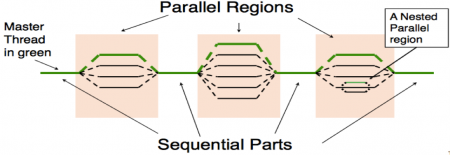
\includegraphics[width=0.7\textwidth]{0.png}
  \caption{Fork-Join Parallelism}
%    \label{doublylog}
\end{figure}


We create threads in OpenMP with the parallel construct. For example, to create a 4 thread Parallel region. Each thread calls $foo(ID, A)$ for $ID = 0$ to 3.


\begin{center}
\begin{lstlisting}[linewidth=17cm]
double A[1000];
omp_set_num_threads(4);
#pragma omp parallel
{
    int ID = omp_get_thread_num();
    foo(ID, A);
}
\end{lstlisting}
\end{center}

\begin{center}
Thread creation: parallel regions
\end{center}

\subsection{Synchronization}
Synchronization is used to impose order constraints and to protect access to shared data. In OpenMP, we have 4 high level synchronization:
\begin{itemize}
    \itemsep-0.2em
    \item critical
    \item atomic
    \item barrier
    \item ordered
\end{itemize}

\subsubsection{Synchronization: critical}
Mutual exclusion: only one thread at a time can enter a {\it critical} region. Example code:
\begin{center}
\begin{lstlisting}[linewidth=17cm]
float result; 
#pragma omp parallel 
{ 
    float B; int i, id, nthrds;
    id = omp_get_thread_num(); 
    nthrds = omp_get_num_threads();
    for(i=id; i<N; i = i+nthrds){ 
        B = foo(i); // expensive computation
    #pragma omp critical
        consume(B, result)
    }
} 
\end{lstlisting}
\end{center}


\subsubsection{Synchronization: atomic}
{\it Atomic} provides mutual exclusion but only applies to the update of a memory location. In the following example code, $foo's$ are run in parallel but {\it r} updated atomically.
\begin{center}
\begin{lstlisting}[linewidth=17cm]
int  n,r;
#pragma omp parallel shared(n,r)
{ 
    for(i=0; i<n; i = i++){ 
    #pragma omp atomic
        r  +=  foo(i); // expensive computation
    }
} 
\end{lstlisting}
\end{center}

\subsubsection{Synchronization: barrier}
{\it Barrier}: Each thread waits until all threads arrive. Example code:
\begin{center}
\begin{lstlisting}[linewidth=17cm]
#pragma omp parallel shared (A, B, C) private(id)
{
    id=omp_get_thread_num();
    A[id] = big_calc1(id); 
    #pragma omp barrier 
    #pragma omp for
    for(i=0;i<N;i++){C[i]=big_calc3(i,A);} 
    #pragma omp for nowait
    for(i=0;i<N;i++){ B[i]=big_calc2(C, i); } 
    A[id] = big_calc4(id); 
}
\end{lstlisting}
\end{center}

\subsubsection{Synchronization: ordered}
The {\it ordered} region executes in the sequential. In the following example code, array {\it a} updated in any order but printed in sequential order
\begin{center}
\begin{lstlisting}[linewidth=18cm]
#pragma omp parallel for
{ 
  for(i=0; i<n; i = i++){ 
    tid = omp_get_thread_num();
    printf("Thread %d updates a[%d]\n", tid, i);
    a[i] += i;
    #pragma omp ordered
    {
      printf("Thread %d prints value of a[%d]=%d\n", 
                tid, i, a[i]);
    }
  }
} 

\end{lstlisting}
\end{center}

\subsubsection{Synchronization: locks}
We also have low level synchronization {\it locks} (both simple and nested).
\begin{itemize}
    \item Simple Lock routines: A simple lock is available if it is unset.
    \begin{itemize}
    \item omp\_init\_lock()
    \item omp\_set\_lock()
    \item omp\_unset\_lock()
    \item omp\_test\_lock()
    \item omp\_destroy\_lock()
    \end{itemize}
    \item Nested Locks: A nested lock is available if it is unset or if it is set but owned by the thread executing the nested lock function.
    \begin{itemize}
    \item omp\_init\_nest\_lock()
    \item omp\_set\_nest\_lock()
    \item omp\_unset\_nest\_lock()
    \item omp\_test\_nest\_lock()
    \item omp\_destroy\_nest\_lock()
    \end{itemize}
\end{itemize}

\subsection{Data Environment and Data Attributes}
All variables declared outside parallel for pragma are shared by default, except for loop index. {\it for} index variable is private. One can selectively change storage attributes for constructs using the following clauses.
\begin{itemize}
    \item shared
    \item private
    \item firstprivate
\end{itemize}

\subsubsection{Private Clausse}
private(var) creates a new local copy of var for each thread. The value is uninitialized and is undefined after the region.

\subsubsection{firstprivate Clausse}
{\it firstprivate} is a special case of private. Initializes each private copy with the corresponding value from the master thread. In the following example, All copies have value of tmp initialized as 0.

\begin{center}
\begin{lstlisting}[linewidth=18cm]
void Foo() 
{ 
    int tmp = 0; 
    #pragma omp for firstprivate(tmp) 
    for (int j = 0; j < 1000; ++j) {
        tmp += j; 
    }
}
\end{lstlisting}
\end{center}

\subsubsection{lastprivate Clausse}
{\it lastprivate} passes the value of a private from the last iteration to a global variable. In the following example, All copies have value of tmp initialized as 0. After the for loop, the variable tmp has the value from the last iteration (i.e. j=99).
\begin{center}
\begin{lstlisting}[linewidth=18cm]
void Foo() 
{ 
    int tmp = 0; 
    #pragma omp for firstprivate(tmp) lastprivate(tmp)
    for (int j = 0; j < 100; ++j) 
        tmp += j; 
        printf("%d\n", tmp);
}
\end{lstlisting}
\end{center}



\section {Find Maximum from N Numbers}
In the first lecture, we mentioned four ways to find maximum from N numbers.

\begin{center}
\begin{tabu} to 0.6\textwidth { | X[l] | X[c] | X[c] |}
 \hline
 & time complexity & space complexity \\
 \hline
 Sequential & $O(N)$ & $O(N)$ \\
 \hline
 Binary Tree  & $O(log(N))$  & $O(N)$  \\
  \hline
 All-pair  & $O(1)$  & $O(N^2)$  \\
  \hline
 Comparison  & $O(1)$  & $O(N^{3/2})$  \\
\hline
\end{tabu}
\end{center}

\subsection{DoublyLog Algorithm}
As we mentioned in the All-pair Algorithm, N numbers can be divided into $\sqrt{N}$ groups. In each group, there are $\sqrt{N}$ numbers. In DoublyLog Algorithm, we further divide every $\sqrt{N}$ group into  $\sqrt{\sqrt{N}}$ sub-groups. We keep doing so until the size of every group is 1 or 2. The height of this tree structure is $log(log(N))$. For each layer, the computing time complexity is $O(N)$. The total time complexity for DoublyLog Algorithm is $O(Nlog(log(N)))$.

\subsection{Cascaded Algorithm}
In Cascaded Algorithm, we combine Sequential Algorithm and DoublyLog Algorithm to reduce the number of processors that we need.

Divide {\it N} numbers into $N/log(log(N))$ groups. Then, in every group, there are $log(log(N))$ numbers. We use Sequential Algorithm to get $N/log(log(N))$ maximum candidates in every group. For these maximum candidates, we use DoublyLog Algorithm.

For Sequential Algorithm, the work complexity is $O(N)$ and time complexity is $log(log(N))$. To select maximum from candidates with DoublyLog Algorithm, the time complexity is  $O(log(log(N)))$ and work complexity is $O(N)$ (There are$N/(log(log(N)))$ groups. Every group has $log(log(N))$ time complexity).

\begin{figure}[!ht]
  \centering
    \includegraphics[width=0.7\textwidth]{1.png}
  \caption{Cascaded Algorithm Model}
%    \label{doublylog}
\end{figure}

\section*{References}
\beginrefs
\bibentry{1}{\sc Leslie Lamport}, A Fast Mutual Exclusion Algorithm(1986).
\bibentry{2}{\sc Michael Merritt}, {\sc Gadi Taubenfeld}, Speeding Lamport?s Fast Mutual Exclusion Algorithm(1991).
\bibentry{3}{\sc Tim Mattson}, A "Hands-on" Introduction to OpenMP (2008).
\bibentry{4} https://github.com/vijaygarg1/UT-Garg-EE382C-EE361C-Multicore
\endrefs


\end{document}





